\chapter{Apêndice: Projeto Olhar do Cinema}

\section{Coleta e seleção de imagens}

\subsection*{Movimento}

\begin{figure}
  \caption[Estudo temático do Movimento]{Estudo temático do Movimento: imagens capturadas da internet e selecionadas em pranchas do \ac{app} Pinterest.}
	\centering
	\includegraphics[height = 5cm]{apendice/movimento/olhar-do-cinema-movimento2.pdf}
	\hfill
	\includegraphics[height = 5cm]{apendice/movimento/olhar-do-cinema-movimento4.pdf}\par

	\par\vspace{3em}
	\includegraphics[width = .35\linewidth]{apendice/movimento/olhar-do-cinema-movimento1.pdf}
\end{figure}

\clearpage

\subsection*{Olhar}

\begin{figure}
  \caption[Estudo temático do Olhar]{Estudo temático do Olhar: imagens capturadas da internet e de autoria própria, seleção no \ac{app} Pinterest.}

	\adjustbox{valign=c}{
		\begin{tikzpicture}
			\clip (0,0) rectangle (4.8cm,4.8cm);
			\node [anchor = south west,inner sep=0pt, outer sep = 0pt]{\includegraphics[height = 5cm]{apendice/olhar/olhar-do-cinema-olhar6.pdf}};
		\end{tikzpicture}
	}\hfill
	\adjustbox{valign=c}{
		\begin{tikzpicture}
			\clip (0,0) rectangle (4.8cm,4.8cm);
			\node [anchor = south west,inner sep=0pt, outer sep = 0pt]{\includegraphics[height = 5cm]{apendice/olhar/olhar-do-cinema-olhar4.pdf}};
		\end{tikzpicture}
	}\hfill
	\adjustbox{valign=c}{
		\begin{tikzpicture}
			\clip (0,0) rectangle (4.8cm,4.8cm);
			\node [anchor = south west,inner sep=0pt, outer sep = 0pt]{\includegraphics[height = 5cm]{apendice/olhar/olhar-do-cinema-olhar5.pdf}};
		\end{tikzpicture}
	}

  \vspace{1em}

	\adjustbox{valign=c}{
		\begin{tikzpicture}
			\clip (0,0) rectangle (4.8cm,4.8cm);
			\node [anchor = south west,inner sep=0pt, outer sep = 0pt]{\includegraphics[width = 5cm]{apendice/olhar/olhar-do-cinema-olhar1.pdf}};
		\end{tikzpicture}
	}\hfill
	\adjustbox{valign=c}{
		\begin{tikzpicture}
			\clip (0,0) rectangle (4.8cm,4.8cm);
			\node [anchor = south west,inner sep=0pt, outer sep = 0pt]{\includegraphics[height = 5cm]{apendice/olhar/olhar-do-cinema-olhar9.pdf}};
		\end{tikzpicture}
	}\hfill
	\adjustbox{valign=c}{
		\begin{tikzpicture}
			\clip (0,0) rectangle (4.8cm,4.8cm);
			\node [anchor = south west,inner sep = 0pt, outer sep = 0pt]{\includegraphics[height = 5cm]{apendice/olhar/olhar-do-cinema-olhar3.pdf}};
		\end{tikzpicture}
	}

  \vspace{1em}

	\adjustbox{valign=c}{
		\begin{tikzpicture}
			\clip (0,0) rectangle (4.8cm,4.8cm);
			\node [anchor = south west, xshift=-1cm,inner sep = 0pt, outer sep = 0pt]{\includegraphics[height = 5cm]{apendice/olhar/olhar-do-cinema-olhar8.pdf}};
		\end{tikzpicture}
	}\hfill
	\adjustbox{valign=c}{
		\begin{tikzpicture}
			\clip (0,0) rectangle (4.8cm,4.8cm);
			\node [anchor = south west,inner sep = 0pt, outer sep = 0pt]{\includegraphics[height = 5cm]{apendice/olhar/olhar-do-cinema-olhar10.pdf}};
		\end{tikzpicture}
	}\hfill
	\adjustbox{valign=c}{
		\begin{tikzpicture}
			\clip (0,0) rectangle (4.8cm,4.8cm);
			\node [anchor = south west,inner sep = 0pt, outer sep = 0pt]{\includegraphics[height = 5cm]{apendice/olhar/olhar-do-cinema-olhar7.pdf}};
		\end{tikzpicture}
	}
\end{figure}

\clearpage

\subsection*{Humano}
\vfill

\begin{figure}
  \caption[Estudo temático do Humano]{Estudo temático do Humano: imagens capturadas da internet e de autoria própria, seleção no \ac{app} Pinterest.}
	\adjustbox{valign=c}{
		\begin{tikzpicture}
			\clip (0,0) rectangle (4.8cm,4.8cm);
			node [anchor = south west, inner sep = 0pt, outer sep = 0pt]{\includegraphics[width = 5cm]{apendice/humano/olhar-no-cinema-humano1.pdf}};
		\end{tikzpicture}
	}\hfill
	\adjustbox{valign=c}{
		\begin{tikzpicture}
			\clip (0,0) rectangle (4.8cm,4.8cm);
			node [anchor = south west, inner sep = 0pt, outer sep = 0pt]{\includegraphics[width = 5cm]{apendice/humano/olhar-do-cinema-humano5.pdf}};
		\end{tikzpicture}
	}

  \vspace{1em}

	\hfil
	\begin{tikzpicture}
		\clip (0,0) rectangle (4.8cm,4.8cm);
		node [anchor = south west, inner sep = 0pt, outer sep = 0pt]{\includegraphics[width = 5cm]{apendice/humano/olhar-do-cinema-humano3.pdf}};
	\end{tikzpicture}
	\hfil

  \vspace{1em}

	\adjustbox{valign=c}{
		\begin{tikzpicture}
			\clip (0,0) rectangle (4.8cm,4.8cm);
			node [anchor = south west, inner sep = 0pt, outer sep = 0pt]{\includegraphics[width = 5cm]{apendice/humano/olhar-do-cinema-humano6.pdf}};
		\end{tikzpicture}
	}\hfill
	\adjustbox{valign=c}{
		\begin{tikzpicture}
			\clip (0,0) rectangle (4.8cm,4.8cm);
			node [anchor = south west, inner sep = 0pt, outer sep = 0pt]{\includegraphics[width = 5cm]{apendice/humano/olhar-do-cinema-humano7.pdf}};
		\end{tikzpicture}
	}
\end{figure}
\vfill

\clearpage

\section*{Cenário}

\vfill
\begin{figure}
  \caption[Estudo temático do Cenário]{Estudo temático do Cenário: imagens capturadas da internet e de autoria própria, seleção no \ac{app} Pinterest.}
	\adjustbox{valign=c}{
		\begin{tikzpicture}
			\clip (0,0) rectangle (4.8cm,4.8cm);
			node [anchor = south west, inner sep = 0pt, outer sep = 0pt]{\includegraphics[width = 5cm]{apendice/cenario/olhar-do-cinema-cenario3.pdf}};
		\end{tikzpicture}
	}\hfill
	\adjustbox{valign=c}{
		\begin{tikzpicture}
			\clip (0,0) rectangle (4.8cm,4.8cm);
			node [anchor = south west, inner sep = 0pt, outer sep = 0pt]{\includegraphics[width = 5cm]{apendice/cenario/olhar-do-cinema-cenario1.pdf}};
		\end{tikzpicture}
	}
  
  \vspace{1em}

	\hfil
	\begin{tikzpicture}
		\clip (0,0) rectangle (4.8cm,4.8cm);
		node [anchor = south west, inner sep = 0pt, outer sep = 0pt]{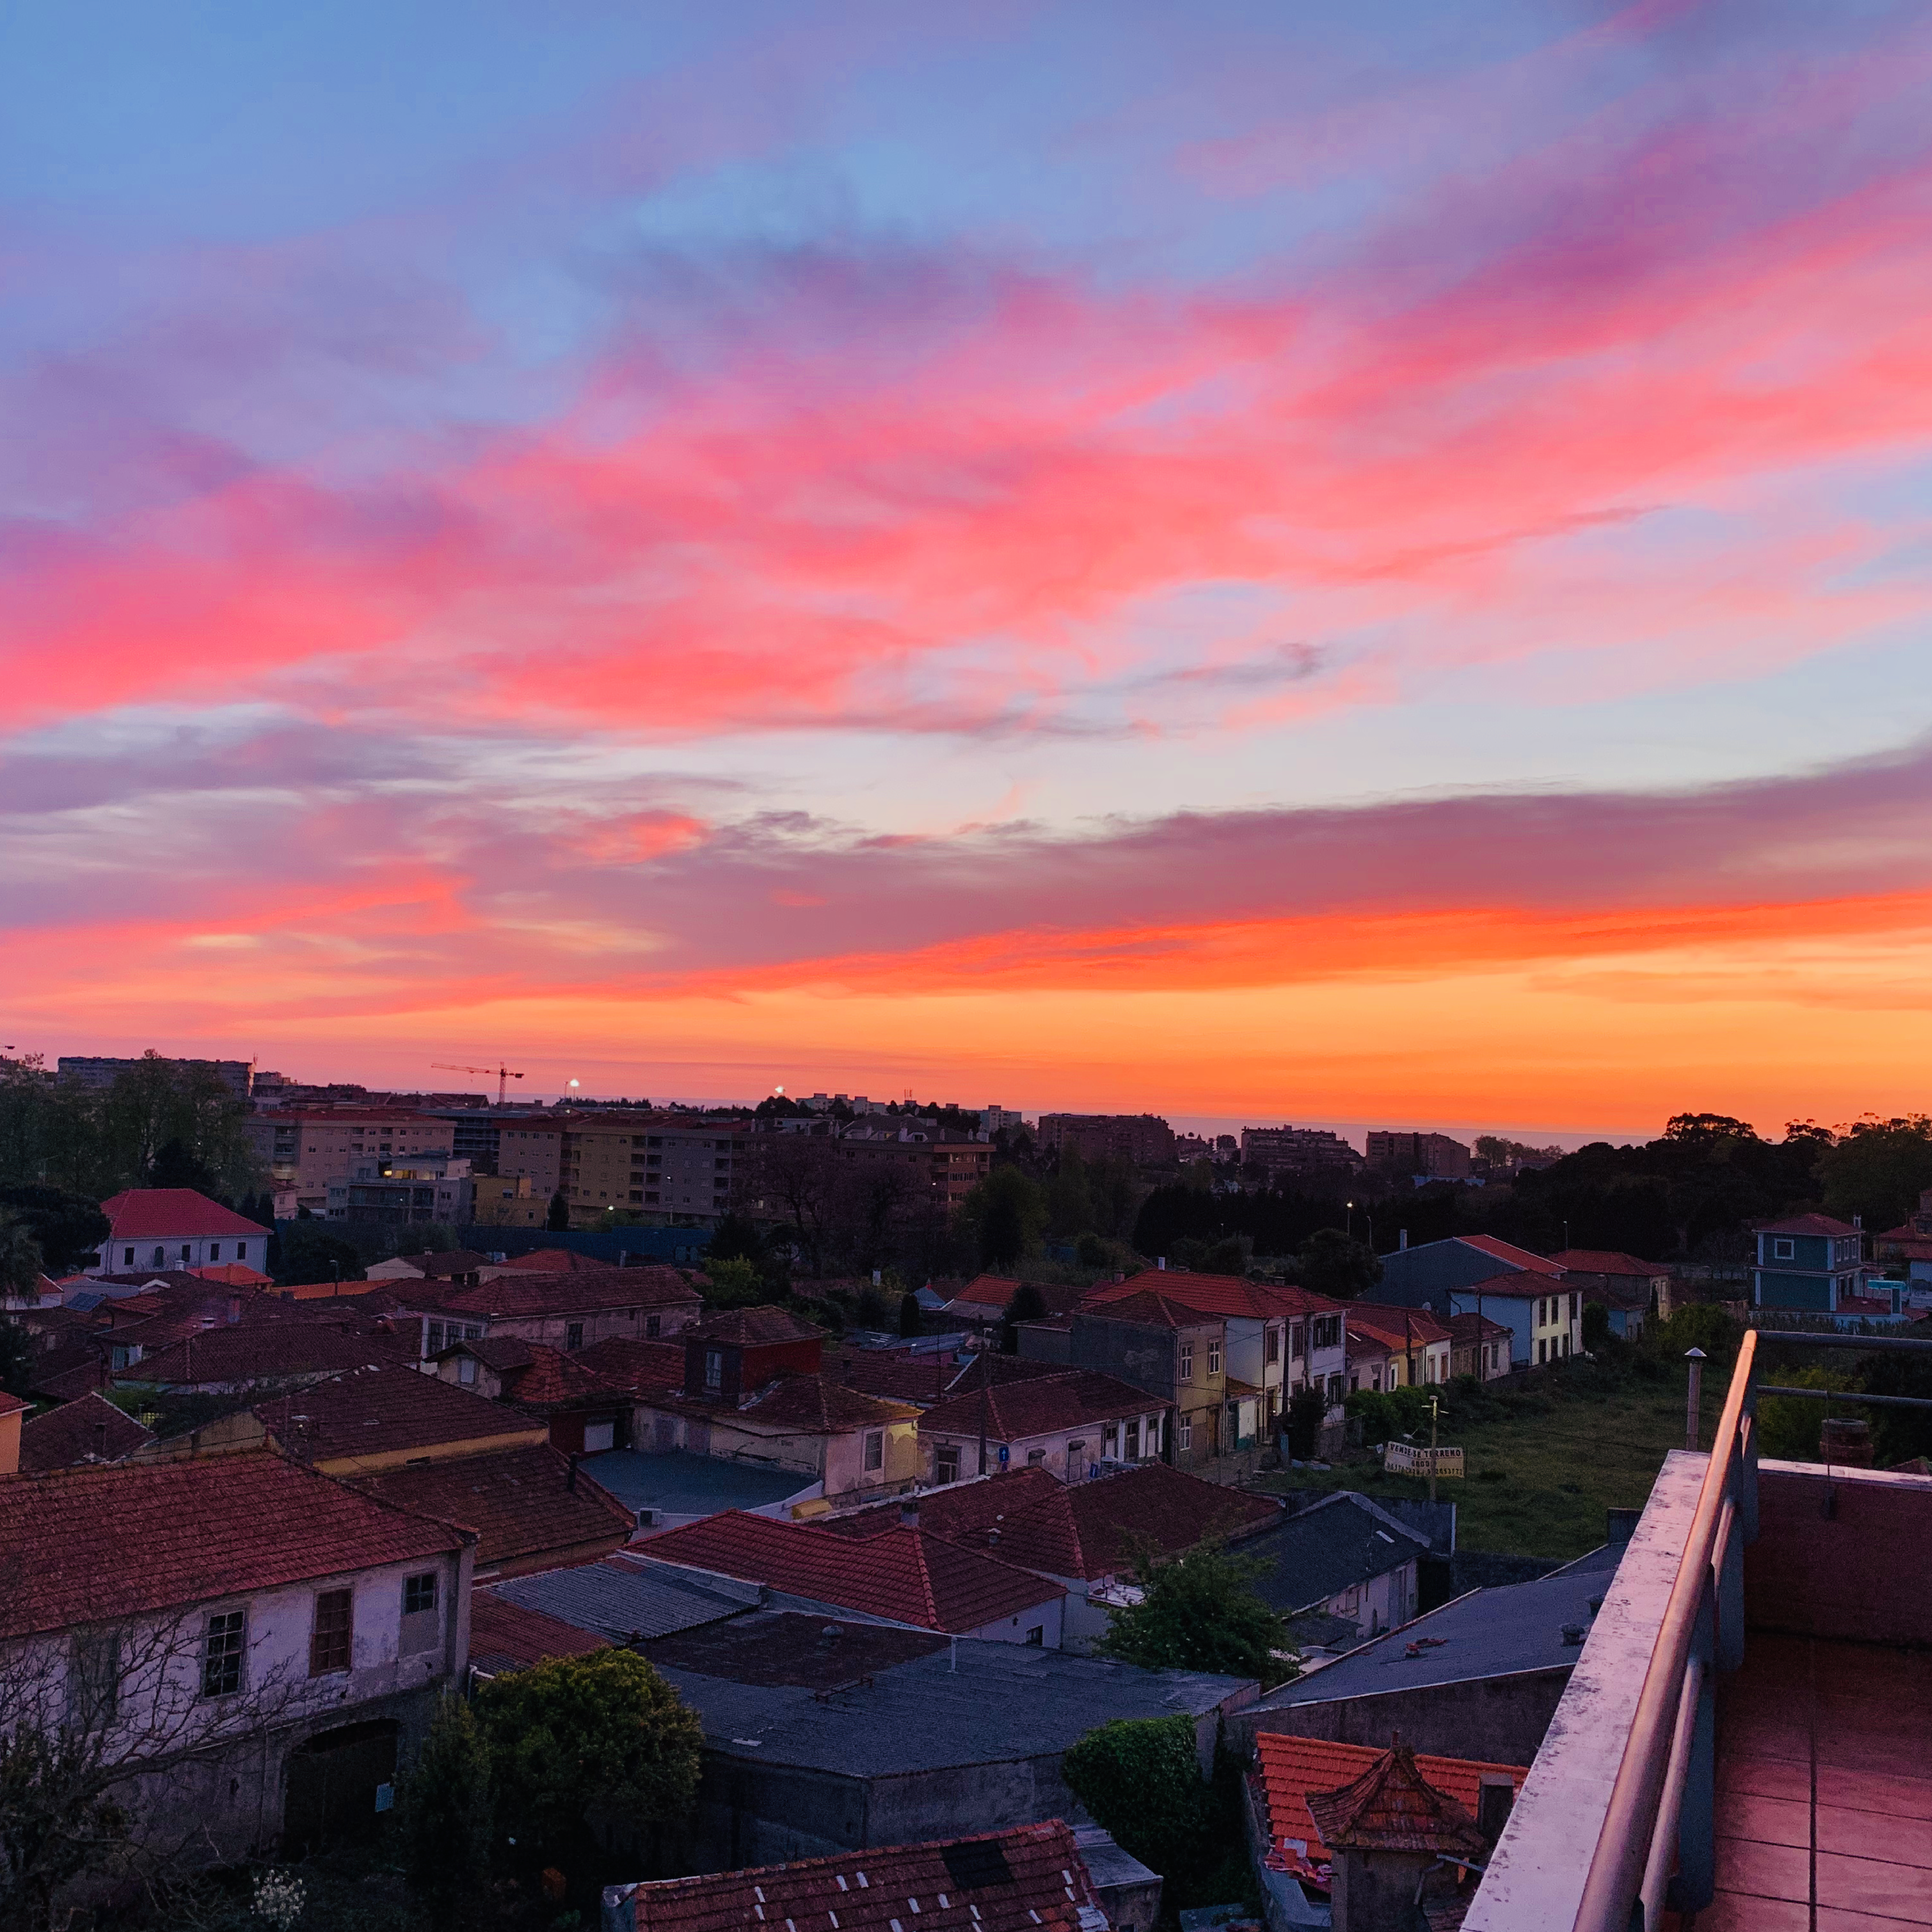
\includegraphics[width = 5cm]{apendice/cenario/olhar-do-cinema-cenario5.pdf}};
	\end{tikzpicture}
	\hfil
  
  \vspace{1em}

	\adjustbox{valign=c}{
		\begin{tikzpicture}
			\clip (0,0) rectangle (4.8cm,4.8cm);
			node [anchor = south west, inner sep = 0pt, outer sep = 0pt, xshift = -1cm]{\includegraphics[height = 5cm]{apendice/cenario/olhar-do-cinema-cenario7.pdf}};
		\end{tikzpicture}
	}\hfill
  \adjustbox{valign=c}{
		\begin{tikzpicture}
			\clip (0,0) rectangle (4.8cm,4.8cm);
			node [anchor = south west, inner sep = 0pt, outer sep = 0pt]{\includegraphics[height = 5cm]{apendice/cenario/olhar-do-cinema-cenario4.pdf}};
		\end{tikzpicture}
	}
	\vfill

\end{figure}

\vfill

\clearpage

\section{Séries e temas em desenvolvimento}

\vfill
\begin{quadro}
	\centering
	\large
	\begin{tabular}{ll}
		\toprule
		Série                                  & Título do trabalho                  \\
		\midrule
		\multirow{4}{*}{Consequências}         & Plongé e contre-plongée             \\
		                                       & Storyboard                          \\
		                                       & Progressão visual                   \\
		                                       & Princípio de afinidade de contraste \\
		\addlinespace
		\multirow{3}{*}{Espaço no Ecrã}        & Espaço profundo e espaço plano      \\
		                                       & Profundidade de campo               \\
		                                       & Rarefação e saturação               \\
		\addlinespace
		\multirow{4}{*}{Humano em Frames}      & Dziga Vertov                        \\
		                                       & Vertigo                             \\
		                                       & Victor Erice                        \\
		                                       & Truffaut                            \\
		\addlinespace
		\multirow{3}{*}{Cenário Fora de Campo} & Cena Méliès                         \\
		                                       & Atlântico norte I e II              \\
		                                       & Atlântico sul I                     \\
		\bottomrule
	\end{tabular}
\end{quadro}

\vfill

\clearpage

\section{Pinturas finalizadas}

\vfill

\begin{figure}
  \caption[Consequências: Plogée e contre-plongée]{\textbf{Consequências} \\ Plongée e contre-plogée}
  \begin{minipage}[b]{.4\linewidth}
    \includegraphics[width = \linewidth]{apendice/pinturas-finalizadas/boudet-eu-quero-ir.pdf}
    \caption*{Eu quero ir, 2020. \\ Série: Me leva. \\ \oleolinho. \\ \artsize{30x20x4}}
  \end{minipage}
  \hfill
  \begin{minipage}[b]{.4\linewidth}
    \includegraphics[width = \linewidth]{apendice/pinturas-finalizadas/boudet-contre-plongee.pdf}
    \caption*{Contre-plongée, 2020. \\ Série: Me leva. \\ \oleolinho. \\ \artsize{20x20x4}}
\end{minipage}
\end{figure}

\vfill

\begin{figure}
  \caption[Consequências: Storyboard]{\textbf{Consequências} \\ Storyboard}
  \begin{minipage}{.35\linewidth}
    \includegraphics[width = \linewidth]{apendice/pinturas-finalizadas/boudet-rolamento-suspenso.pdf}
    \caption*{Rolamento suspenso, 2021. \\ Série: Movimento de câmera. \\ \oleolinho. \\ \artsize{37.5x37.5x4}}
  \end{minipage}\hfill
  \begin{minipage}{.55\linewidth}
    \includegraphics[width = \linewidth]{apendice/pinturas-finalizadas/boudet-under-the-bed.pdf}
    \caption*{\emph{Under the bed}, 2021. \\ Série: Movimento de câmera. \\ \oleolinho. \\ \artsize{57.5 x 82}}

    \includegraphics[width = .6\linewidth]{apendice/pinturas-finalizadas/boudet-retrato-na-parete.pdf}
    \caption*{Retrato na parede, 2021. \\ Série: Movimento de câmera. \\ \oleolinho. \\ \artsize{20x20x4}}
  \end{minipage}
\end{figure}

\vfill

\begin{figure}
  \caption[Espaço no ecrã: Espaço profundo]{\textbf{Espaço no ecrã} \\ Espaço profundo}
  \begin{minipage}{.45\linewidth}
	\includegraphics[width = \linewidth]{apendice/pinturas-finalizadas/boudet-caminho-cor-de-rosa.pdf}
  \caption*{Caminho cor de rosa, 2022. \\ Sére: Espaço no ecrã. \\ \oleo. \\ \artsize{20x20x3.5}}
\end{minipage}\hfill
\begin{minipage}{.45\linewidth}
	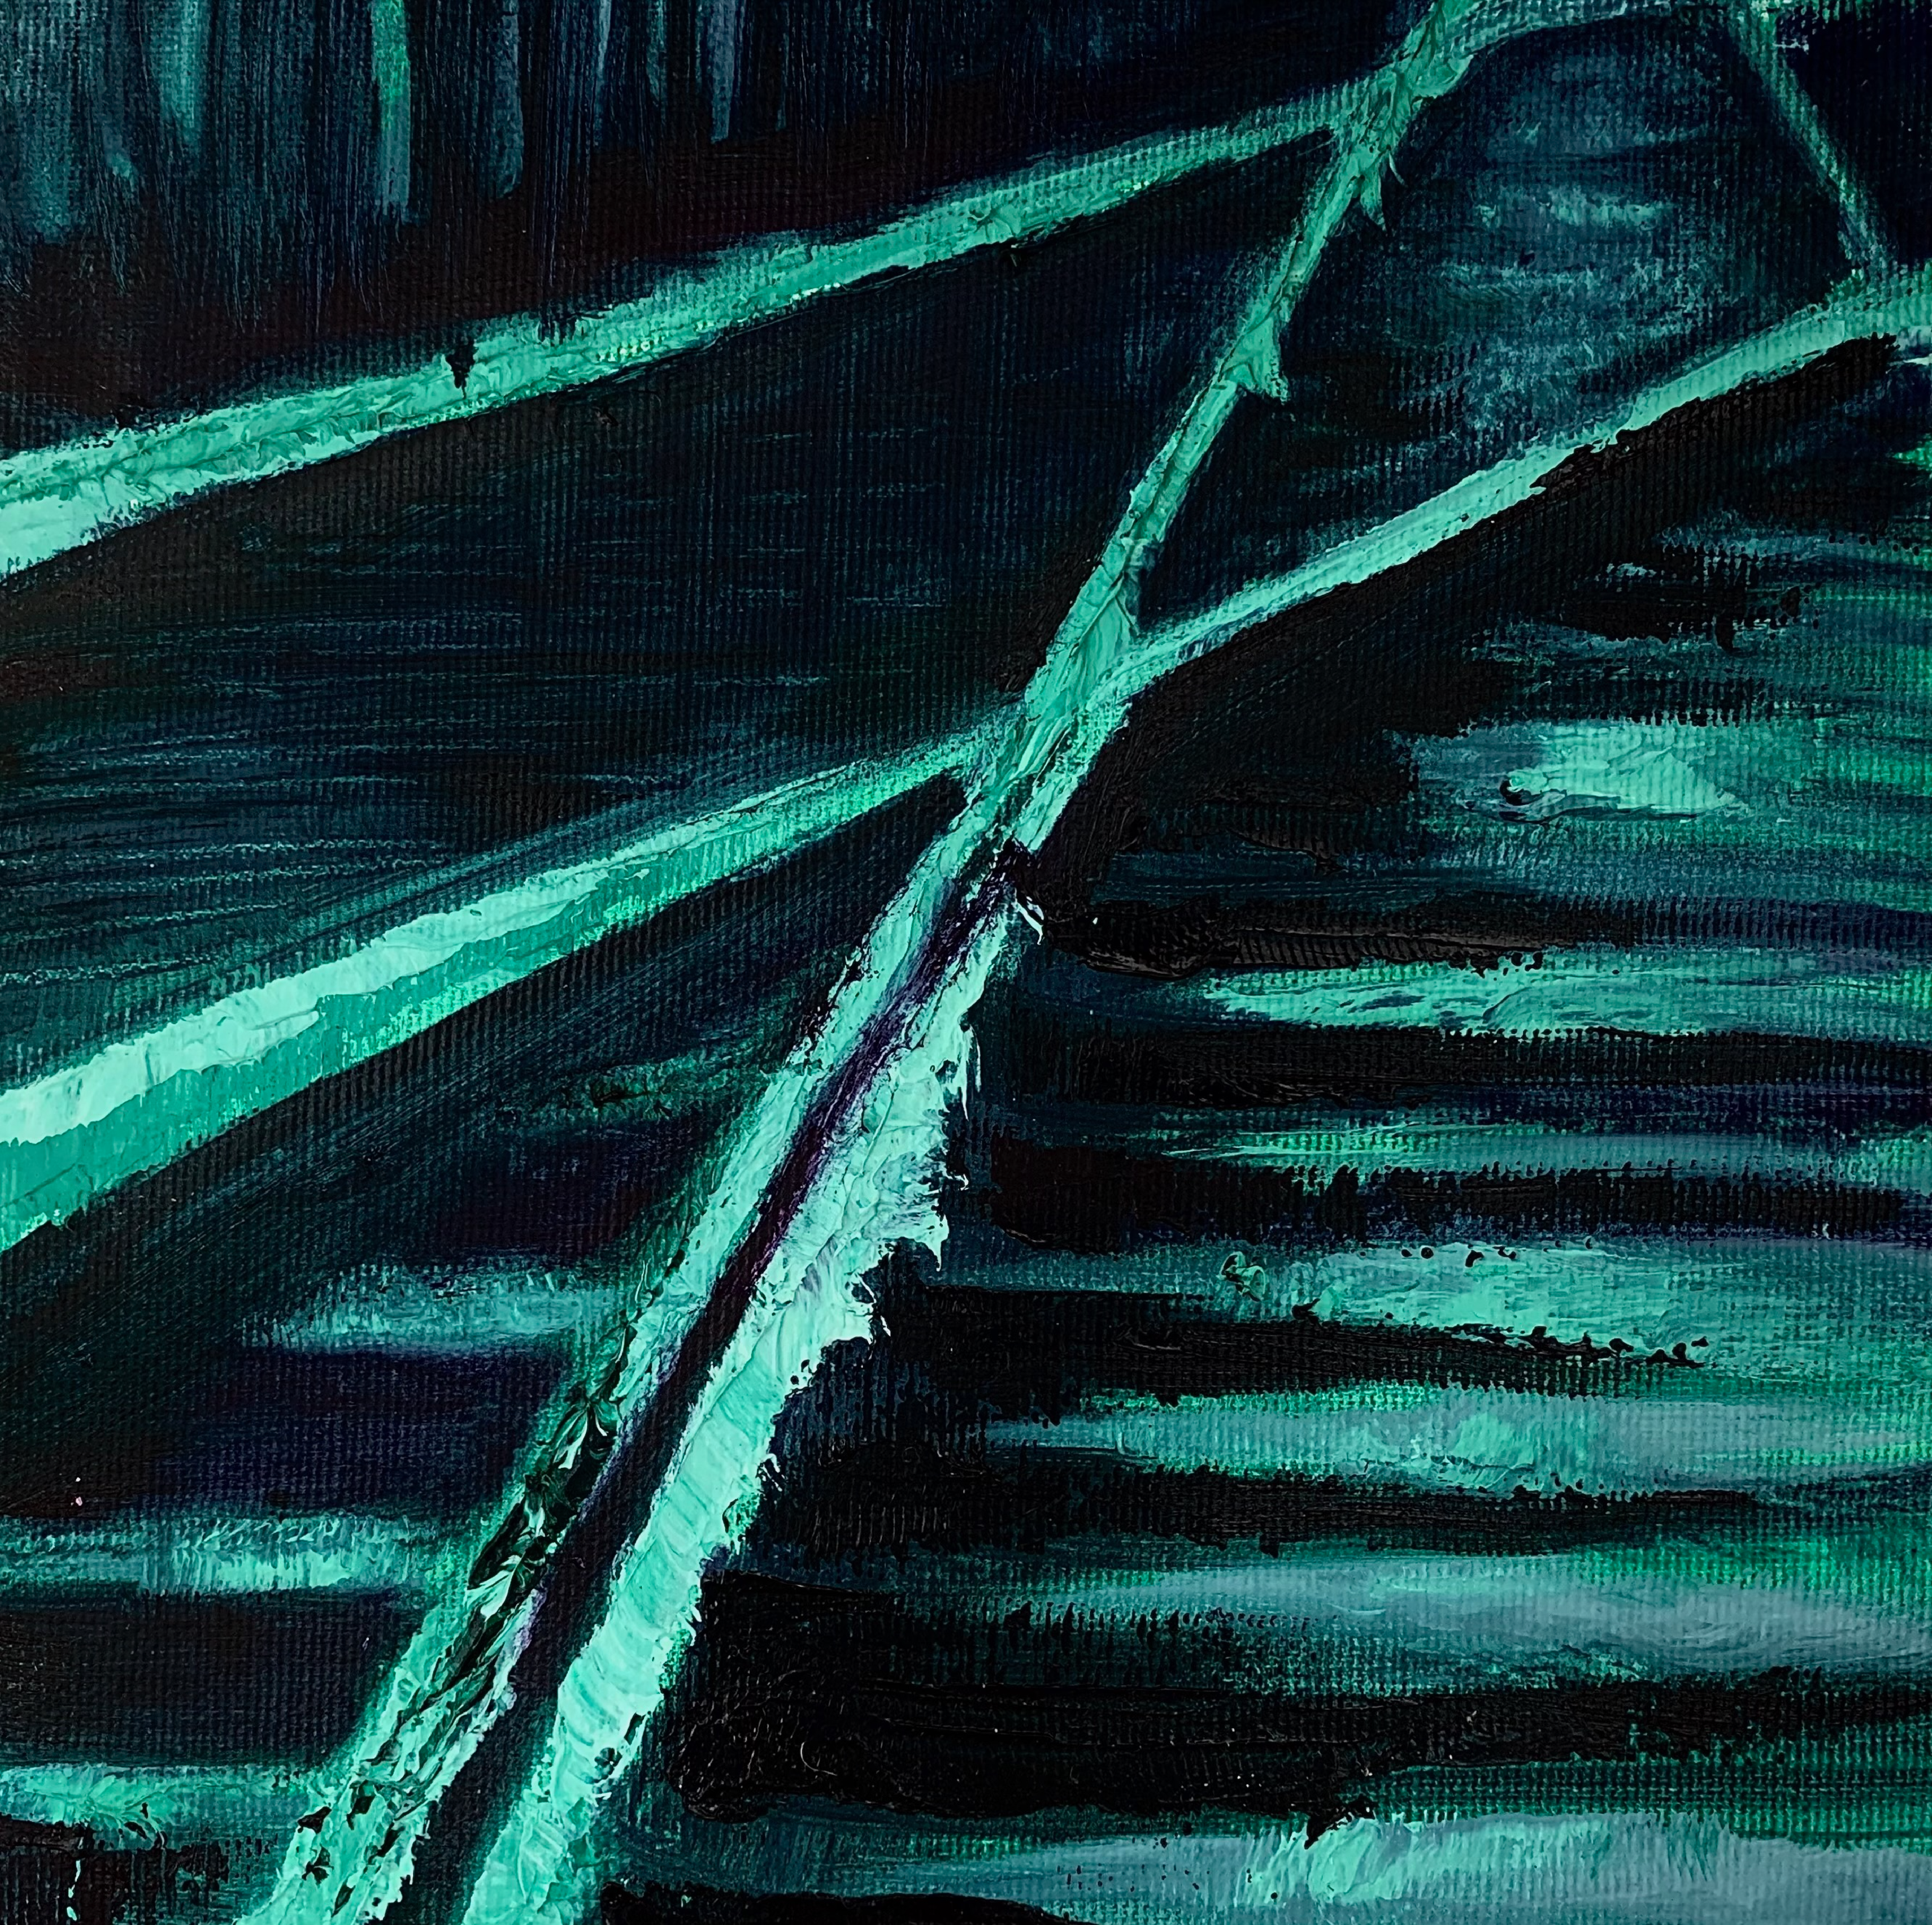
\includegraphics[width = \linewidth]{apendice/pinturas-finalizadas/boudet-espaco-profundo.pdf}
  \caption*{Espaço profundo I, 2022. \\ Série: Espaço no ecrã. \\ \oleo. \\ \artsize{20x20x3.5}}
\end{minipage}
\end{figure}

\vfill

\begin{figure}
  \caption[Espaço no ecrã: Profundidade de campo]{\textbf{Espapço no ecrã} \\ Profundidade de campo}
  \begin{minipage}[b]{.7\linewidth}
	\includegraphics[width = \linewidth]{apendice/pinturas-finalizadas/boudet-profundidade-i.pdf}
  \caption*{Profundidade de campo I, 2022 \\ Série: Espaço no ecrã. \\ \oleolinho. \artsize{30x30x3.5}}
\end{minipage}

\vspace{2em}

\begin{minipage}{.91\linewidth}
\begin{minipage}{.3\linewidth}
	\includegraphics[width = \linewidth]{apendice/pinturas-finalizadas/boudet-profundidade-campo-i-detalhe1.pdf}
\end{minipage}
\hfill
\begin{minipage}{.3\linewidth}
	\includegraphics[width = \linewidth]{apendice/pinturas-finalizadas/boudet-profundidade-campo-i-detalhe2.pdf}
\end{minipage}
\hfill
\begin{minipage}{.3\linewidth}
	\includegraphics[width = \linewidth]{apendice/pinturas-finalizadas/boudet-profundidade-campo-i-detalhe3.pdf}
\end{minipage}
\caption*{Profundidade de campo I, 2022 \\ Série: Espaço no ecrã. \\ Detalhes.}
\end{minipage}
\end{figure}

\clearpage

\begin{figure}[t]
  \caption[Humano em frames: Dziga Vertov]{\textbf{Humano em frames} \\ Dziga Vertov}
  \begin{minipage}[t]{.45\linewidth}
	\includegraphics[width = .7\linewidth]{apendice/pinturas-finalizadas/boudet-dziga-vertov-i.pdf}
  \caption*{Dziga Vertov I, 2022. \\ Série: Humano em frames. \\ \oleo. \\ \artsize{20x20x3.5}}
\end{minipage}
\begin{minipage}[t]{.45\linewidth}
	\includegraphics[width = \linewidth]{apendice/pinturas-finalizadas/boudet-dziga-vertov-ii.pdf}
  \caption*{Dziga Vertov II, 2022. \\ Série: Humano em frames. \\ \oleolinho. \\ \artsize{40x40x3.5}}
\end{minipage}
\end{figure}

\vfill

\begin{figure}[b]
  \caption[Humano em frames: Victor Erice]{\textbf{Humano em frames} \\ Victor Erice}
  \begin{minipage}[t]{.45\linewidth}
	\includegraphics[width = .7\linewidth]{apendice/pinturas-finalizadas/boudet-victor-erice-i.pdf}
  \caption*{Victor Erice I, 2022. \\ Série: Humano em \emph{frames}. \\ \oleo. \\ \artsize{20x20x3.5}}
\end{minipage}
\begin{minipage}[t]{.45\linewidth}
	\includegraphics[width = \linewidth]{apendice/pinturas-finalizadas/boudet-victor-erice-iI.pdf}
  \caption*{Victor Erice II, 2022. \\ Série: Humano em \emph{frames}. \\ \oleolinho. \\ \artsize{40x40x3.5}}
\end{minipage}
\end{figure}

\vfill

\clearpage

\begin{figure}[t]
  \caption[Cenário fora de campo: Atlântico]{\textbf{Cenário fora de campo} \\ Atlântico}
  \begin{minipage}[b]{.3\linewidth}
	\includegraphics[width = \linewidth]{apendice/pinturas-finalizadas/boudet-atlantico-sul-i.pdf}
  \caption*{Atlântico sul I, 2022. \\ Série: Cenário fora de campo. \\ \oleolinho. \\ \artsize{15x15x3.5}}

	\includegraphics[width = \linewidth]{apendice/pinturas-finalizadas/boudet-atlantico-norte-i.pdf}
  \caption*{Atlântico norte I, 2022. \\ Série: Cenário fora de campo. \\ \oleolinho. \\ \artsize{15x15x3.5}}
\end{minipage}\hfill
\begin{minipage}[b]{.65\linewidth}
	\includegraphics[width = \linewidth]{apendice/pinturas-finalizadas/boudet-atlantico-norte-ii.pdf}
  \caption*{Atlântico norte II, 2022. \\ Série: Cenário fora de campo. \\ \oleolinho. \\ \artsize{50x50x3.5}}
\end{minipage}
\end{figure}


\begin{figure}
  \flushright
\begin{minipage}[l]{.4\linewidth}
  \caption[Cenário fora de campo: Cena Méliès]{\textbf{Cenário fora de campo} \\ Cena Méliès}
	\includegraphics[width = \linewidth]{apendice/pinturas-finalizadas/boudet-cena-melies-i.pdf}
  \caption*{Cena Méliè I, 2022. \\ Série: Cenário fora de campo \\ \oleolinho. \\ \artsize{20x20x3.5}}
\end{minipage}
\end{figure}

\clearpage

% \begin{figure}
% 	\includegraphics[width = .4\linewidth]{apendice/pinturas-finalizadas/boudet-vertigo-i.pdf}
% 	\includegraphics[width = .4\linewidth]{apendice/pinturas-finalizadas/boudet-vertigo-ii.pdf}
%
% 	\includegraphics[width = .4\linewidth]{apendice/pinturas-finalizadas/boudet-vertigo-iii.pdf}
% \end{figure}

